\newpage
\section{Qusilinear and Nonlinear First Order PDEs}
\textbf{Date:} Sep 14, 2021
\subsection{quasilinear PDEs and conversation laws}
Last time, we were looking at first order, quasilinear, scalar PDEs
\[
    \sum_j A_j(x,u)\partial_j u + b(x,u) = 0.
\]
We saw that our characteristics have to consider both $x$ and $u$. We need to solve the characteristic system 
\[
    \begin{cases}
        \dot x = A(x,u)\\ 
        \dot u = -b(x,u)
    \end{cases}
\]
to get a local solution. Because characteristics carry information about $x$ and $u$, there was no prohibition against characteristics intersecting. If our initial data is $u|_\Sigma=u_0$, then the noncharacteristic condition becomes
\[
    A(x_0, u_0(x_0)) \cdot N  \neq 0 \quad \text{on }\Sigma.
\]

\begin{remark}
    The condition of being noncharacteristic depends both on the surface and on the initial data on the surface. So the {\it problem} is noncharacteristic, rather than the surface (until we have fixed set of initial data).
\end{remark}

Now since we can just consider $\Sigma = \{t=0\}$, the model problem is
\[
\begin{cases}
    \partial_t u + \sum_j A_j(x,u) \partial_j u + b(x,u) = 0\\
    u|_{t=0}=u_0
\end{cases}
\]
Since we already using $t$, let's use $s$ as the parameter along the characteristics. We have 
\[
    \begin{cases}
        \dot s = 1\\
        \dot x = A(x,u)\\
        \dot u = -b(x,u)
    \end{cases}
\]
The first equation tells us that we can choose $s=t$. This corresponds to a dimensionality reduction of our problem.

\begin{example}
    [Conservation Law]
    A special case of this is what we call conservation laws: 
    \[
        u_t + \sum_j\partial_j F_j(u) = 0.
    \]
    We can equivalently write this as 
    \[
        u_t + \sum_j F_j'(u) \partial_j u = 0.
    \]
    Using the first form is not important for scalar equations, but it is for scalar systems because it is not always the case that we can write the second version with a divergence term.

    The first version is called \textbf{density flux notation}. THis is because the $u_t$ tells how the density of some quantity changes in time, and the flux term, $\partial_jF_j(u)$, tells you how the mass is moving with velocity $F_j'(u).$
\end{example}

\subsection{Burgers' equation}
\begin{example}
    [Burgers' equation] The simplest quasilinear problem is the Burgers' equation 
    \[
        \begin{cases}
            u_t+uu_x = 0\\
            u|_{t=0} = u_0.
        \end{cases}
    \]
    This equation seems simple, but it ends up being a model problem for more complicated
equations. Here are the characteristics:
    \[
        \begin{cases}
            \dot x = u\\
            \dot u =0.
        \end{cases}
    \]
    Thus the characteristics are $x(t) = x_0 + tu_0(x_0)$. Hence, the characteristics may intersect as follows: 
    \begin{figure}[H]
        \centering
        \begin{tikzpicture}[framed]
            \draw[thick](-3,0) -- (3,0);
            \node at (3,0.3) {$\Sigma = \{t=0\}$};
            \draw[->, thick, orange] (-2,0) -- (1.5,3) node[above] {$u_0(x_0)$};
            \draw[->, thick, orange] (2,0) -- (-2,2.5) ;
        \end{tikzpicture}
        \end{figure}

    How would we choose our dat aso the lines don't intersect? If $u_0$ is increasing , the picture looks like this: 
    \begin{figure}[H]
        \centering
        \begin{tikzpicture}[framed]
            \draw[thick](-3,0) -- (3,0);
            \draw[->, thick, orange] (-2,0) -- (-3,1.5);
            \draw[->, thick, orange] (-1,0) -- (-1,2);
            \draw[->, thick, orange] (0.5,0) -- (1,2);
            \draw[->, thick, orange] (2,0) -- (4,2);
        \end{tikzpicture}
        \end{figure}
    So we get a global solution forward in time, but we don't get a global solutions backward in time. So the only global solutions are constant.
\end{example}

\begin{remark}
    In physics, we expect there to be {\it causality}. That is, we expect the future to be determined by the past but not the past to be determined by the future. Later we will see what we will do after the point where characteristics intersect.
\end{remark}

\begin{example}
    Let' give an equation for $u_x$: 
    \[
        u_{tx}+uu_{xx} + u^2_x =0.
    \]
    If we write $u_x=v$, then this equation is just talking about the derivative along the characteristics: 
    \[
        (\partial_t + u \partial_x)v + v^2 = 0.
    \]
    We may also write this as
    \[
        \dot v + v^2 = 0,
    \]
    where the dot is the derivative along the characteristic. This equation tells us how the slope of the solution is evolving. If $v_0>0$, the slope decreases toward $0$. However, if $v_0<0$, we get finite time blow-up.
    
    \vspace{1em}
        \begin{minipage}{0.45\textwidth}
        \begin{tikzpicture}[framed]
            \draw[->, thick](-1,0) -- (4,0);
            \draw[->, thick](0,-2) -- (0,2);
            \draw[scale=1, domain=0:4, smooth, variable=\x, blue] plot ({\x}, {2/(\x+2)});
            \draw[scale=1, domain=0:1.5, smooth, variable=\x, blue] plot ({\x}, {2/(\x-2)});
            \node at (-.5,1) {$v_0$};
            \node at (3, -2) {finite time blow-up};
        \end{tikzpicture}
    \end{minipage}
    \begin{minipage}{ 0.45\textwidth}
        \centering
        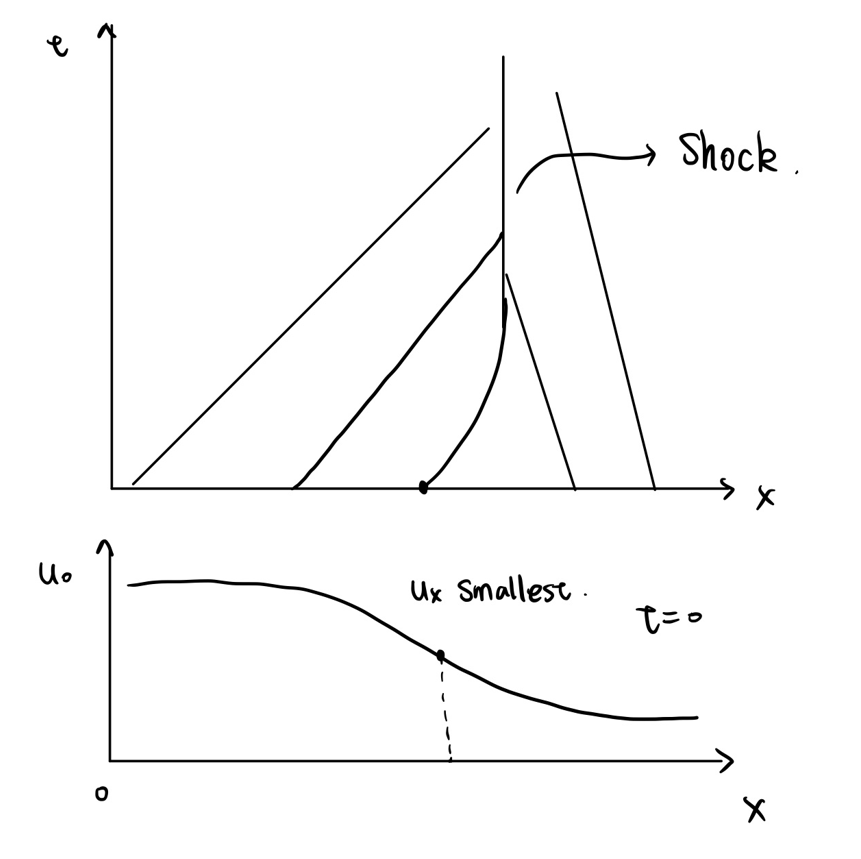
\includegraphics[width=0.9\textwidth]{pics/6-1.png}
    \end{minipage}
    \vspace{1em}

    The smallest slope means the fastest blow-up. Suppose the initial data $u_0$ is decreasing, so we will get intersections of characteristics.Suppose the initial data $u_0$ is decreasing, so we will get intersections of characteristics.   Because things intersect, there is no unique way to continue the equation. Here, we have a \textbf{shock}, or a jump discountinuity. We will see later how to find what the equation fo the shock curve looks like. 

    Conservation laws is still a very active area, with a number of hard problems.

\end{example}

\subsection{Fully nonlinear problems}

We now look at PDEs of the form 
\[
    \begin{cases}
        F(x,u,\partial u) = 0\\ 
        u|_{\Sigma}= u_0,
    \end{cases}
\]
where the dependence on $\partial u$ is nonlinear.  Where do we start? Before, we had a vector
field that let us interpret the equation using a directional derivative.

Let’s look at the linearized equation: Suppose we have not just a solution but a 1-
parameter family of solutions $u^h$ to our problem with solution $v^h$ to our linearized given by
\[
    \frac d {dh} u^h = v^h.
\]
Differentiate the equation with respect to $h$ to get the linearized equation: 
\[
    0=\frac{\partial}{\partial h} F\left(x, u^{h}, \partial u^{h}\right)=F_{u} \cdot v^{h}+\sum_j F_{p_{j}} \cdot \partial_{j} v^{h},
\]
where we write $F=F(x,u,p)$ and $p=(p_1,\dots, p_n)$.
This linearized equation is linear transport equation. So we get a vector field $A_j = F_{p_j}(x,u, \partial u)$. We should try to use this vector field to find characteristics. Our equation looks like 
\[
\begin{cases}
    \dot x_j = F_{p_j}(x,u, \partial u)\\
    \dot u = \dots
\end{cases}
\]
The first equation depends on $\partial u$, so we may try to add an equation $\dot \partial u = \dots$. But then we  would get $\partial^2 u$ in this equation, and we would be in the same situation. How do we get past this issue?

This is trivial since 
\[
    \dot u = \sum_j \partial_j u \cdot \dot x_j = \sum_j F_{p_j}(x,u, \partial u) \cdot \partial_j u.
\]
We also have 
\begin{align*}
    0 &=\partial_{x_j} F(x, u, \partial u) \\
    &=F_{x_{j}}(x, u, \partial u)+F_{u}(x, u, \partial u) \partial_{j} u+\underbrace{\sum_k F_{p_{k}}(x, u, \partial u) \partial_{k} \partial_{j} u}_{=\sum_{k}\dot x_k \partial_k\partial_{j} u = \dot{\partial_j u}}
\end{align*}
Therefore, the characteristic equations are: 
\[
\begin{cases}
    \dot x_j = F_{p_j}(x,u,\partial u)\\
    \dot u = \sum_j F_{p_j}(x,u, \partial u) \cdot \partial_j u\\
    \dot{\partial_j u} = -F_{x_j}(x,u,\partial u) - F_u(x,u, \partial u)\cdot \partial_j u.
\end{cases}
\]
Or we can write it as: 
\begin{equation}
    \label{eq:chractereqs}
\begin{cases}
    (a) \, \dot x_j(t) = F_{p_j}(x,z,p)\\
    (b) \, \dot z(t) = \sum_j F_{p_j}(x,z,p) \cdot p^j u\\ 
    (c) \, \dot p_j(t) = -F_{x_j}(x,z,p) - F_z(x,z,p)\cdot p_j
\end{cases}
\end{equation}

In fact, we have proved that 
\begin{theorem}
    [Structure of chracteristic ODE] Let $u\in \con^2(U)$ solve the nonlinear, first order PDE in $U$. Assume $x(\cdot)$ solves the 1.(a), where $p(\cdot) = Du(x(\cdot)), z(\cdot) = u(x(\cdot))$. Then $p(\cdot)$ solves the 1.(c) and $z(\cdot)$ solves the 1.(b). 
\end{theorem}


Now we may ask what is the initial data for this system \eqref{eq:chractereqs}? We had $x(0) = x_0$ and $u(0) = u_0$ before, but now we have 
\[
\begin{cases}
    x(0) = x_0\\
    u(0) = u_0\\
    \partial u(0) = ?
\end{cases}
\]

We need the information of all the derivatives of $u$ at $x_0$. In particular, we need both $n-1$ tangential derivatives to $\Sigma$ and 1 normal partial derivative to $\Sigma$. If we frame this in the tangnet space, we wan t the tangent derivative $\partial'=(\partial_1, \partial_2, \ldots,\partial_{n-1} )$ and the normal derivative $\partial_n$. We know $\partial'$, but what about $\partial_n$? 
\begin{figure}[H]
    \centering
    \begin{tikzpicture}[framed]
        \draw[thick] plot [smooth, tension =0.8]
        coordinates {(-0.2,3) (0.1,2) (0.4,1) (-0.3,0) (0.2,-1)};
        \node at (0.1,1) {$x_0$};
        \node at (0.2, 3) {$\Sigma$};
        \draw[->, thick, orange] (0.4,1) -- (1.4,1) node[above] {$\partial_n$};
        \draw[->, thick, orange] (0.4,1) -- (0.4,0) node[right] {$\partial'$};
    \end{tikzpicture}
\end{figure}
We know that 
\[
    F(x_0, u_0 , \partial'u_0 , \partial_n u) = 0,
\]
so we would like to solve for $\partial_n u$. This tells us that 
\[
    \partial_n u = G(x_0, u_0, \partial'u_0),
\]
for some function $G$. We can do this if 
\[
    F_{p_n}(x_0, u_0, \partial' u_0, p_n) \neq 0.
\]
If we didnt put our equation in this special frame, this condition reads as 
\[
    F_p(x_0,u_0,p)\cdot N \neq 0,
\]
the condition that the equation is noncharacteristic.

\begin{remark}
    What if this question has more than 1 solution? We may not get uniqueness; the answer may depend on our choice here of initial data.
\end{remark}

